\documentclass{beamer}
\usetheme{Singapore}
%\setbeamercolor{structure}{fg=red}
\usepackage{upgreek}
\usepackage{color}
%\def\magyarOptions{hyphenation=huhyphn}
%\usepackage{ae,aecompl}
%\usepackage[T1]{fontenc}
\usepackage[utf8]{inputenc}
%\usepackage[hungarian]{babel}
\usepackage{gensymb}
\usepackage{pgfplots}
\usepackage{pst-plot}
\usepackage{tikz}
\usepgfplotslibrary{external}
\tikzexternalize
\usepackage{xcolor}
\usepackage[version=3]{mhchem}

\normalfont
\title{Potentiometric scanning electrochemical microscopic mapping of the distributed Belousov-Zhabotinsky oscillating reaction}
\subtitle{1st International Conference on Reaction Kinetics, Mechanisms and Catalysis}
\author
{András Kiss\\
\hfill \\
}
\institute
{
  %\inst{1}%
  Department of General and Physical Chemistry\\
  University of Pécs\\
  \hfill \\

  \includegraphics[width=0.14\textwidth]{pte_logo.eps}\\
  June 6--9, 2018 / Budapest, Hungary
}

\date[]

\begin{document}
\frame{\titlepage}  


\begin{frame}
	\centering
	\includegraphics[width=0.6\textwidth]{secm_english.eps}
	\frametitle{\underline{S}canning \underline{E}lectro\underline{c}hemical \underline{M}icroscope}
\end{frame}

\begin{frame}
	\centering
	\includegraphics[width=0.8\textwidth]{koros.eps}
	\frametitle{\underline{B}elousov-\underline{Z}habotinsky reaction}
\end{frame}

\begin{frame}
	\centering
	\includegraphics[width=0.5\textwidth]{zygote.jpeg}\includegraphics[width=0.5\textwidth]{davinci.jpg}
	\frametitle{The BZ-reaction as a model for pattern formation}
\end{frame}

\begin{frame}
	\centering
	\includegraphics[width=0.5\textwidth]{turing.jpg}\includegraphics[width=0.5\textwidth]{morpho.eps}

	\frametitle{,,The chemical basis of morphogenesis''}
\end{frame}

\begin{frame}
	\centering
	\emph{,,Only the future can say whether such reactions will become more than a laboratory curiosity.''}

\vspace{1cm}

Endre Kőrös -- 1972 (Oscillating in Chemical Systems. II.)
%	\frametitle{Kémiai hullámok \emph{Xenopus} embrióban}
\end{frame}



\begin{frame}
	\centering
	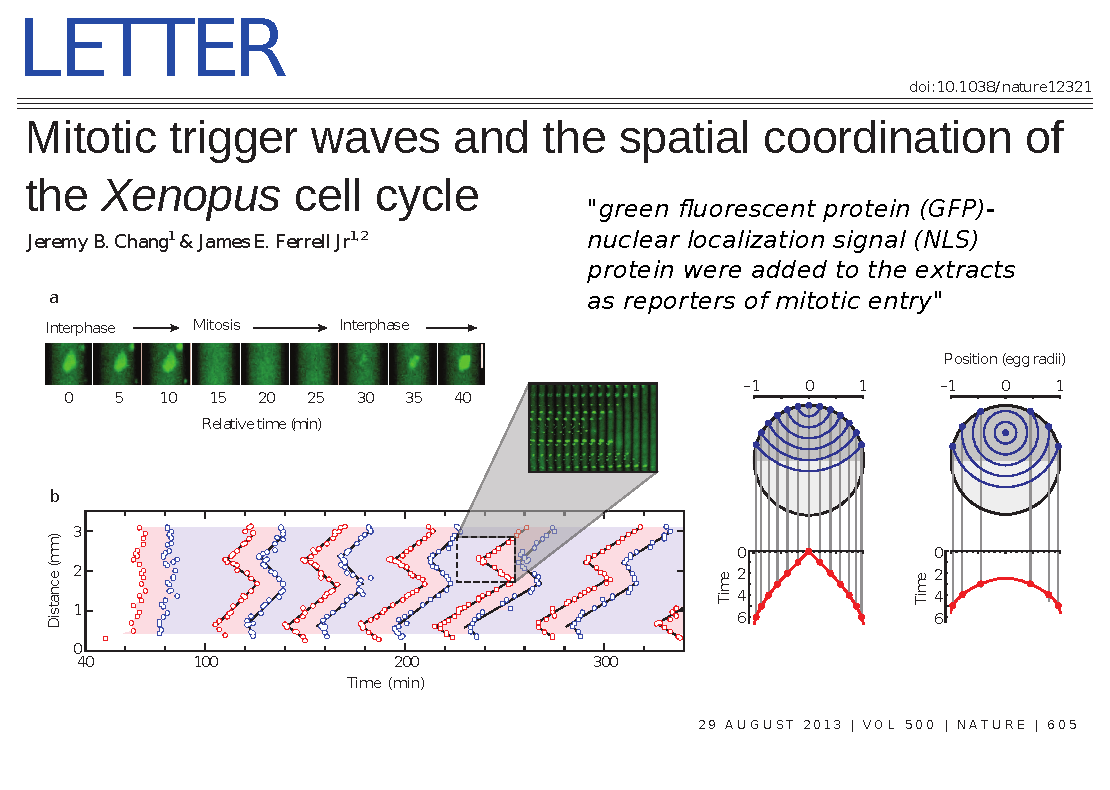
\includegraphics[width=0.8\textwidth]{chang.eps}
	\frametitle{Chemical waves in \emph{Xenopus} embryo}
\end{frame}

\begin{frame}
	\centering
	\includegraphics[width=0.8\textwidth]{setup1.jpg}
	\frametitle{Stationary measurement}
	\framesubtitle{Method}
\end{frame}


\begin{frame}
\frametitle{Stationary measurement}
\framesubtitle{The measured parameters}
\begin{columns}[T] % align columns
\begin{column}{.48\textwidth}

\centering
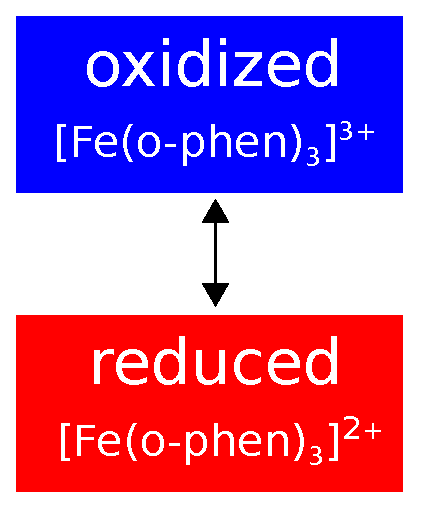
\includegraphics[width=0.6\textwidth]{ferroin.eps}

Ferroin redox--indicator

\end{column}%
\hfill%
\begin{column}{.48\textwidth}
%\color{blue}\rule{\linewidth}{4pt}
\centering


%\footnotesize
\begin{equation*}
        E=E^\theta + \frac{RT}{z_iF} \ln \frac{[Fe^{3+}]}{[Fe^{2+}]}
\end{equation*}
%\normalsize

Nernst--equation
\end{column}%
\end{columns}
\end{frame}

\begin{frame}
\frametitle{Oscillation of the \textcolor{red}{[Fe$^{2+}$]}/\textcolor{blue}{[Fe$^{3+}$]} ratio}
\framesubtitle{Explained by the FKN--mechanism}
\tiny
\begin{align}
\tiny
\ce {BrO3^- + Br- + CH2(COOH)2 + 3 H+ &-> 3 BrCH(COOH)2 + 3 H2O}\\
\ce {BrO3^- + \textcolor{red}{\ce {Fe^2+}} + CH2(COOH)2 + 5 H+ &-> BrCH(COOH)2 + 4 \textcolor{blue}{\ce {Fe^3+}} + 3 H2O}\\
\ce {4 \textcolor{blue}{\ce {Fe^3+}} + BrCH(COOH)2 + 2 H2O &-> Br- + 4 \textcolor{red}{\ce {Fe^2+}} + HCOOH + 2 CO2 + 5 H+}\\
\ce {CH2(COOH)2 + 6 \textcolor{blue}{\ce {Fe^3+}} + 2 H2O &-> 6 \textcolor{red}{\ce {Fe^2+}} + HCOOH + 2 CO2 + 6 H+}\\
\ce {3 BrO3^- + 5 CH2(COOH)2 + 3 H+ &-> 3 BrCH(COOH)2 + 2 HCOOH + 4 CO2 + 5 H2O}
\large
\end{align}
\large
\end{frame}


\begin{frame}
	\centering
	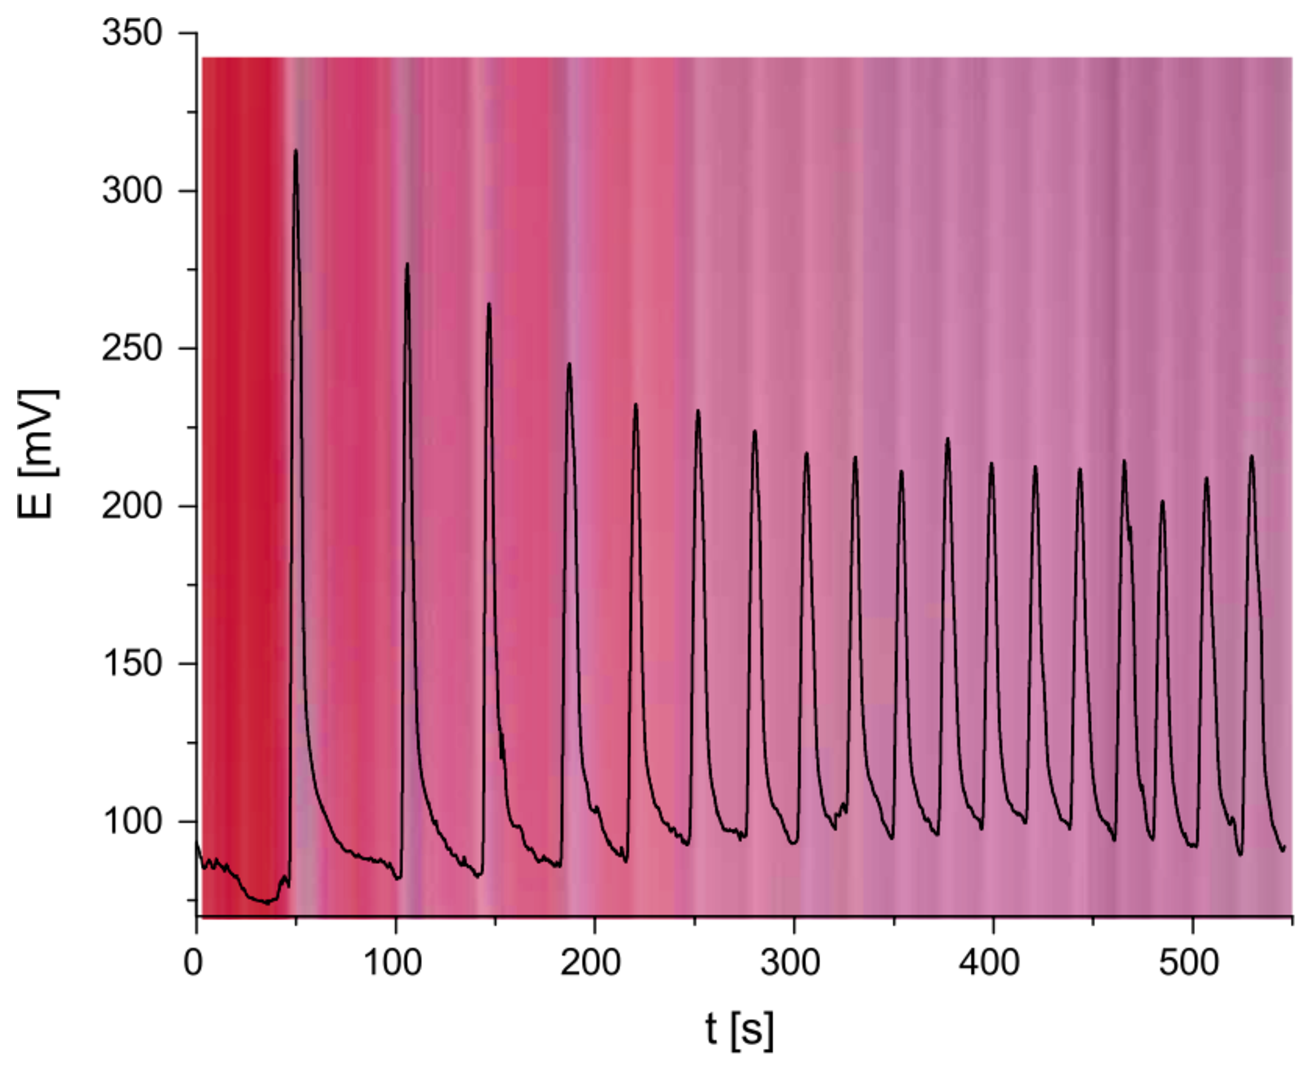
\includegraphics[width=0.8\textwidth]{pontszerumeres.eps}
	\frametitle{Stationary measurement}
	\framesubtitle{Result}
\end{frame}



\begin{frame}
	\centering
	\includegraphics[width=0.8\textwidth]{setup_photo.jpg}
	\frametitle{SECM scanning}
	\framesubtitle{Measurement setup}
\end{frame}

\begin{frame}
	\centering
	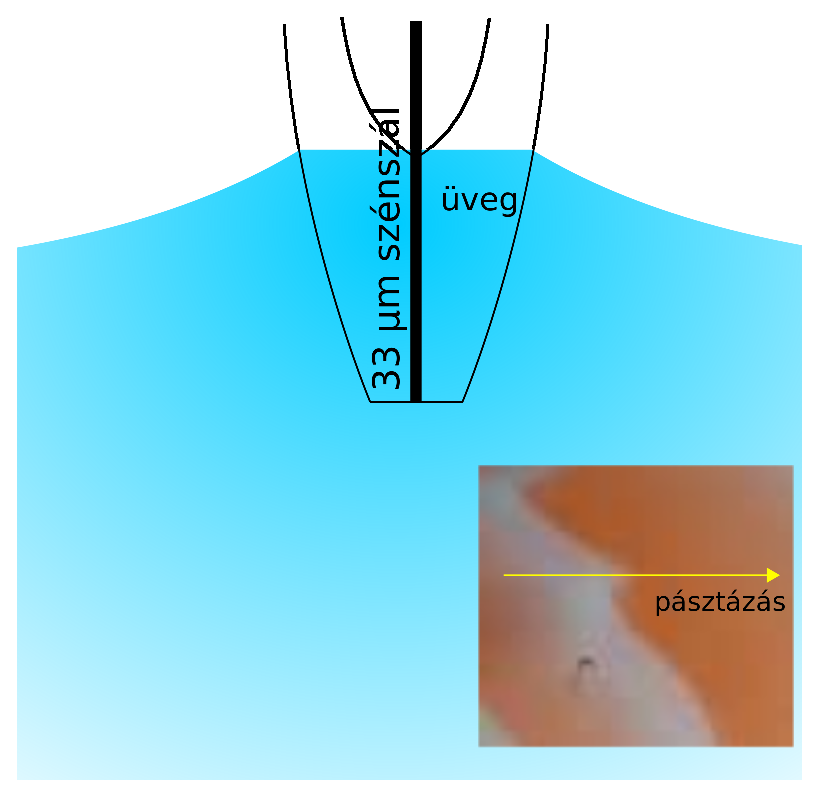
\includegraphics[width=0.6\textwidth]{szigeteles1.eps}
	\frametitle{Convective disturbance}
	\framesubtitle{Conventional carbon microelectrode in the reaction mixture}
\end{frame}

\begin{frame}
	\centering
	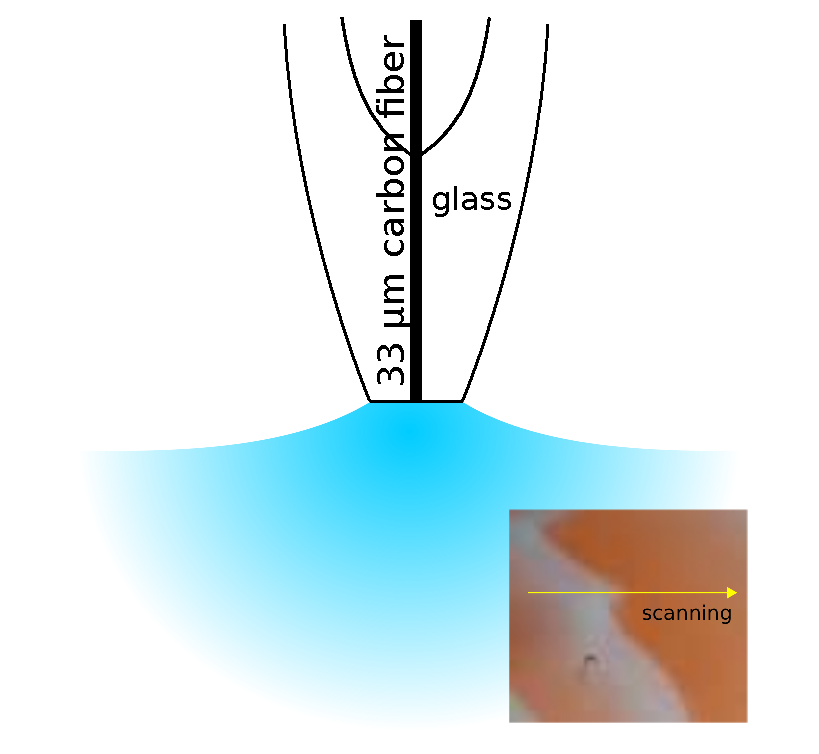
\includegraphics[width=0.6\textwidth]{szigeteles2.eps}
	\frametitle{Convective disturbance}
	\framesubtitle{Conventional carbon microelectrode on the surface of the reaction mixture}
\end{frame}

\begin{frame}
	\centering
	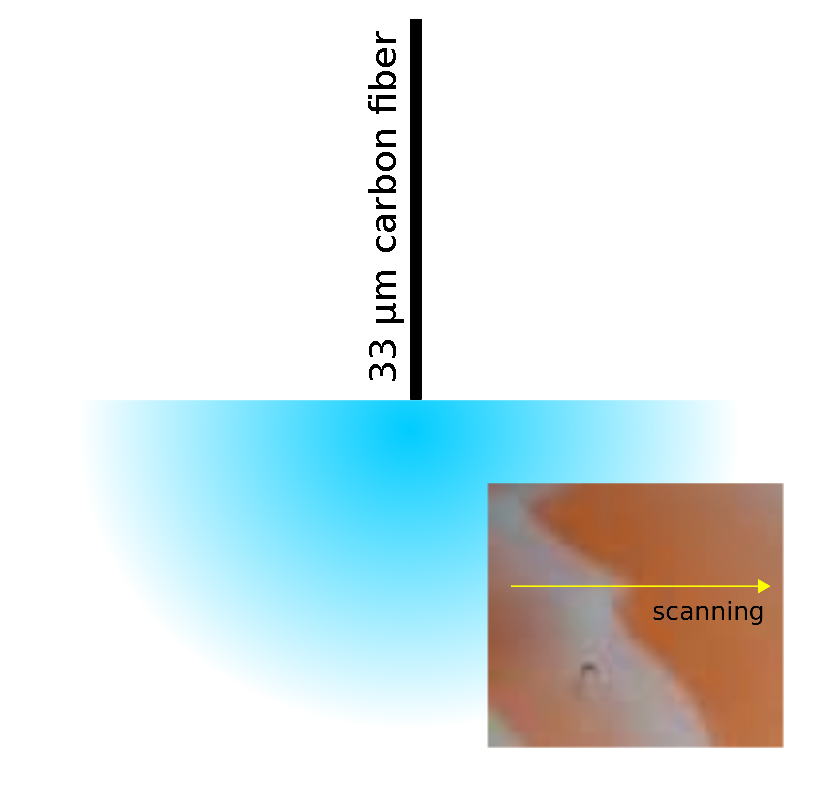
\includegraphics[width=0.6\textwidth]{szigeteles3.eps}
	\frametitle{Convective disturbance}
	\framesubtitle{Uninsulated carbon fiber on the surface of the reaction mixture (d = 33 $\upmu$m)}
\end{frame}

\begin{frame}
	\centering
	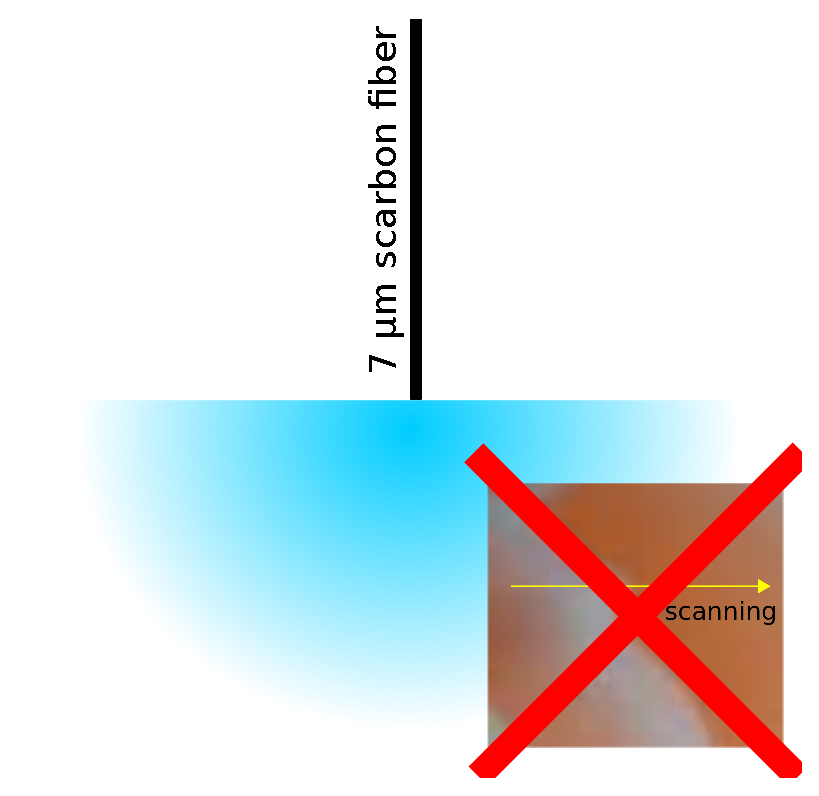
\includegraphics[width=0.6\textwidth]{szigeteles4.eps}
	\frametitle{Convective disturbance}
	\framesubtitle{Uninsulated carbon fiber on the surface of the reaction mixture (d = 7 $\upmu$m)}
\end{frame}

\begin{frame}
	\centering
	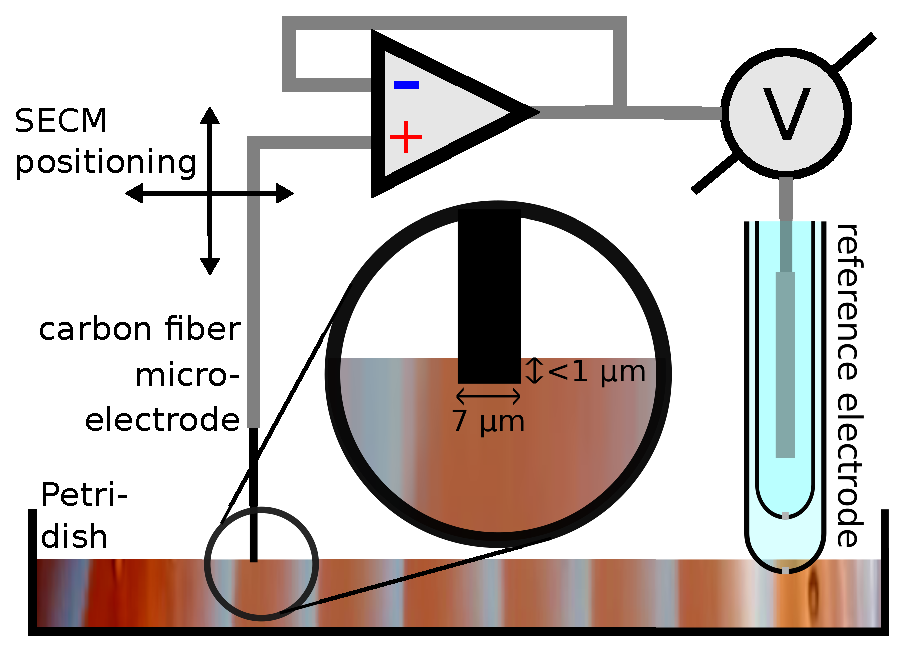
\includegraphics[width=0.8\textwidth]{setup.eps}
	\frametitle{SECM scanning}
	\framesubtitle{Measurement setup}
\end{frame}

\begin{frame}
	\centering
	\includegraphics[width=0.6\textwidth]{grabs.png}
	\frametitle{SECM scanning}
	\framesubtitle{Convective disturbance}
\end{frame}

\begin{frame}
	\centering
	\includegraphics[width=0.8\textwidth]{spacetime_ill.eps}
	\frametitle{SECM scanning}
	\framesubtitle{Evaluating the result}
\end{frame}

\begin{frame}
	\centering
	\includegraphics[trim = 15mm 60mm 0mm 30mm, clip, width=0.5\textwidth, angle=-90]{spacetime.eps}
	\frametitle{SECM scanning}
	\framesubtitle{Result}
\end{frame}

\begin{frame}
	\frametitle{SECM scanning}
	\framesubtitle{Result}

\begin{table}
\tiny
\label{table:stats}
\centering
\begin{tabular}{r c c c c c}
Wave \# & t, s & E, mV & x, mm & v, $\upmu$m/s \\
 \hline
 \hline
 3&\begin{tabular}{c}47\\67\\80\end{tabular}&\begin{tabular}{c}957\\978\\977\end{tabular}&\begin{tabular}{c}1.4\\6.4\\8.6\end{tabular}&218.8\\
 \hline
 6&\begin{tabular}{c}99\\114\\133.5\end{tabular}&\begin{tabular}{c}968\\975\\1027\end{tabular}&\begin{tabular}{c}1\\4.8\\7.6\end{tabular}&191.3\\
 \hline
 7&\begin{tabular}{c}148.5\\171\\181.5\end{tabular}&\begin{tabular}{c}1052\\1127\\1059\end{tabular}&\begin{tabular}{c}1.6\\7.2\\8.8\end{tabular}&218.18\\
 \hline
 9&\begin{tabular}{c}200\\219.5\\234.5\end{tabular}&\begin{tabular}{c}1016\\1074\\1016\end{tabular}&\begin{tabular}{c}1.4\\6.2\\8\end{tabular}&191.3\\
 \hline
 12&\begin{tabular}{c}253.5\\268\\287\end{tabular}&\begin{tabular}{c}1060\\1120\\1053\end{tabular}&\begin{tabular}{c}0.4\\5.2\\7.4\end{tabular}&208.96\\
\end{tabular}
\end{table}
\end{frame}


\begin{frame}
	\frametitle{Conclusion}
	\centering
\begin{itemize}
\item A small enough scanning probe will not disturbe the BZ--reaction.

\item Using the SECM, the advantages of the optical and electrochemical methods can be combined, and spatially resolved chemical images can be obtained about the distributed BZ--reaction.

\item Replacing the carbon fiber with an ion-selective microelectrode, bromide-ion activity and pH could be mapped.

\item The surface scanning could be used in other cases, where minimal disturbance is required.
\end{itemize}
\end{frame}


\begin{frame}
	\frametitle{Acknowledgements}
	\centering
	Most of the experiments were performed by my first supervised student, \textbf{Szilárd Szili} (Chemistry BSc.).
\end{frame}

\begin{frame}
	\centering
	Thank you for your attention.

%	\includegraphics[width=0.8\textwidth]{thanks.jpg}

\end{frame}



\end{document}
